\chapter{Drupal: case study and research questions}
\chaptermark{Case study and research questions}
\label{chapter:case-study}

Drupal is a Free/Libre Open Source content management framework released in 2001. It provides a robust platform for the development of web applications and currently powers more than 2\% of websites worldwide. This percentage includes well-known websites with complex architectures and high loads of traffic, such as whitehouse.gov, mtv.co.uk and economist.com. Section \ref{sec:what-is-drupal} provides an introduction to Drupal as a technology, as well as to a series of basic technical notions in order to clarify the vocabulary used by the Drupal community.

Drupal represents one of the most well-known examples of the phenomenon of Commons-Based Peer Production. As the slogan of the project reflects --- ``come for the software, stay for the community" --- , Drupal cannot be understood without considering its community, which is the main focus of this study. The Drupal community has experienced significant growth over the years: there are currently more than 1.3 million people registered on the main collaboration platform, among which more than 105,000 have actively contributed to the project. The community is also highly active offline, holding numerous events of different scopes every week worldwide. Section \ref{sec:drupal-history} offers an overview of key moments in the history of the project and the community in order to contextualise the case study. Certain fundamental aspects for this research, such as the growth of the community or the strong presence of a ``do-ocratic" culture, are more extensively discussed in sections \ref{sec:growth-community} and \ref{sec:do-ocracy} respectively. Finally, the chapter concludes by presenting the research questions tackled in this study in section \ref{subsubsec:state-art:drupal:case-study}.

\section{What is Drupal?}
\label{sec:what-is-drupal}

Drupal is a FLOSS content management framework: a software designed to build dynamic websites, web applications, web resources and web services, providing a set of common functionalities that can be adapted and extended \parencite{drupal-wap:2014:Online}. It is based on the programming language PHP\footnote{PHP is a FLOSS scripting language, extensively employed in web development \parencite{php:2017:Online}.} and the source code is licensed under a GPL license\footnote{\label{fn-gpl} As presented in sections \ref{subsec:hacker} and \ref{subsec:bazaar}, a GPL license is a popular license within FLOSS communities that fulfils the criteria of the Free Software Foundation to protect users' freedoms.}.

\begin{figure}[H]
	\centering
	\includegraphics[scale=0.3]{img/druplicon.png}
	\caption[Druplicon: Drupal's logo]%
    {``Druplicon" is the main logo of Drupal. It depicts a drop with an infinity symbol to resemble eyes. Retrieved \nth{4} November 2014, from \url{https://www.drupal.org/node/9068}, under a GPL version 2 license.}
	\label{druplicon}
\end{figure}

When a ``fresh" installation of Drupal is made (see figure \ref{fresh-drupal}), the developer will find a set of basic functionalities that are typically available in Content Management Systems\footnote{A Content Management System (CMS) is a software designed for the creation and modification of digital contents. Drupal presents hybrid characteristics between web application frameworks and CMS. Other examples of popular FLOSS Content Management Systems are Wordpress or Joomla.}. For example, to manage the registration of users, to define types of content --- such as a blog post and a wiki page ---, and to define permissions to access and create such content.

Using Drupal terminology, this process consists of installing Drupal core: the main codebase. The core is composed of tens of modules\footnote{For example version 7.43 has 40 modules, or version 8.04 counts 64 modules. The number of modules which form part of the core is relevant, since it is an indicator of the complexity of the project. These aspects will be widely discussed in chapter \ref{chapter:core-system}.} that provide basic functionalities. A module is a collection of files, including source code, to provide certain functionalities. In addition, the installation of Drupal core would include a set of themes. A theme is a collection of files, including source code, to define the presentation layer of the website\footnote{This distinction is made to fulfil a basic software design pattern known as Model-View-Controller, in which the logic is separated from the way the information is processed and represented.}.

\begin{figure}[H]
	\centering
	\includegraphics[scale=0.45]{img/fresh_drupal.png}
	\caption[Drupal site after a ``fresh" installation]%
    {A Drupal site after a ``fresh" installation. At this point the system provides a set of basic functionalities, provided by Drupal \textit{core} modules, and the contents are presented with a specific style, as defined by the default theme ``bartik".}
	\label{fresh-drupal}
\end{figure}

Although these basic functionalities provided by the core are  important to develop any web-based system --- they can be seen as its kernel\footnote{This refers to a similar comparison as that made for the kernel of an operating system in section \ref{subsec:bazaar}: the hearth of the system.} --- the power of Drupal resides in its extendibility. For example, when developing a website using Drupal, a developer will typically carry out a process of configuration using these basic functionalities to fulfil part of the requirements of a project. For instance, the programmer may need to create a set of web pages and to link them in a menu at the top of the page.

Nevertheless, programmers will also commonly need to extend Drupal sites with more functionalities that are not provided by Drupal core. For example, they may need to embed a Twitter timeline\footnote{This is a basic example chosen for illustrative purposes. Indeed, it is so basic that they could also fulfil the same functionality requirement using only \textit{core} modules.} in the site. At this point, the developer will have two options. The first option is to look for a certain module, or a combination, which once properly configured and combined with other modules, fulfil that specific functionality requirement. For example, the developer might download and install a module named ``Twitter block\footnote{See \url{https://www.drupal.org/project/twitter_block}.}". These modules are known as \textit{contributed}\footnote{Within the Drupal community, the term \textit{contributed} typically refers specifically to those projects shared at Drupal.org, the main collaboration platform. Nevertheless, a developer could decide to share a project in a different place, and this could also be considered ``\textit{contributed}" in case they use a FLOSS license. Nevertheless, in this thesis the term ``\textit{contributed}" will be used for projects shared on the main collaboration platform, unless otherwise stated.} modules. They can be seen as ``plugins" that extend the functionalities provided by the core. These modules are shared and collaboratively maintained on the Internet by groups of Drupalistas. This pool of \textit{contributed} projects represents a rich set of digital commons which has been key for the success and popularity of Drupal. The richness of this system is captured in the popular motto within the community: ``There is a module for that!" \parencite{abbott2016learning}, referring to the extensive amount of modules that enable Drupalistas to build most of the functionalities without having to code.

Drupal's main collaboration platform offers a large pool of more than 20,000 modules and nearly 2,500 themes under a GPL license\footnote{A dynamic directory on the main collaboration platform accessed on \nth{15} February 2017, from \url{https://www.drupal.org/project/project_module} and \url{https://www.drupal.org/project/project_theme}, lists 20,005 modules and 2,417 themes classified as ``full projects": whose quality standards have been reviewed and passed by the community.}, known within the community as \textit{contributed} Drupal projects. In addition, the platform provides tools to share and improve projects collectively, as a digital commons. Furthermore, Drupalistas exchange information about how to use them to achieve certain functionalities. Thus, in a similar manner as someone may share cooking recipes (e.g. explaining them to a neighbour or posting them online), Drupalistas focus on sharing instructions on how to configure modules or a combination of them.

The second option for programmers would be to develop their own module to use Twitter services and embed the timeline into Drupal. In this case they would need to interact with Drupal's core to create what in Drupal is known as a \textit{custom} module. The interaction with the core system is carried out through a ``hook system". Hooks are the main means by which modules interact with Drupal core\footnote{This example refers to the classical architecture of Drupal, up to version 7. The ``hook system" was removed during the development of the latest version of Drupal, which was a source of tension in the community, as will be explained in section \ref{subsec:d7-d8}. From a software engineering point of view, the system is not considered to follow best practices, since it does not follow well-established paradigms such as Object Oriented Programming. However, it provides fast and simple ways to develop functionalities, since it facilitates the ability to ``hook" into any event of the system.} \parencite{drupal-hooks:2016:Online}. Hooks also provide entry points to change and add new functionalities. In addition, a module can define its own hooks, to enable other modules to interact with it. \textit{Custom} modules are often created for a particular use that is specific for a functionality of the site. Due to this specificity, in many cases they are not shared. However, some Drupalistas attempt to publish them in Drupal.org and apply for a process to make them part of the pool of \textit{contributed} projects in Drupal.org\footnote{Chapter \ref{sec:custom-to-contrib} provides an extensive overview and analysis of how quality control processes such as these are organised and how they have changed over time.}. In other cases, some Drupalistas may share modules in repositories that are not part of the official collaboration platform, such as GitHub\footnote{Github (\url{https://github.com/}) is a popular hosting service of distributed version control systems as those described in section \ref{subsec:floss-tools}.}.

The previous paragraphs introduced some of the basic steps that someone may take when using Drupal as a technical product. Nevertheless, Drupal cannot be understood simply as a product, but rather a communitarian project. Drupal is maintained and developed by a community of more than one million users, from which more than 105,000 have actively contributed to the project \parencite{drupal-getting-involved:2017:Online}. It is precisely in the community where this research places its main focus. Drupal is one of the most-well known cases of Commons-Based Peer Production, with a large global community that self-organises using an open development model with the aim of constantly improving the project and including the latest web technologies.

With the aim of highlighting how CBPP communities organise themselves and have been able to scale up their self-organisational processes, this study is focussed on Drupal as an instance of an extreme case study of CBPP. Thus, this study addresses the emergence of organisational structures, their changes, and the organisational dynamics of this global community which continues to undergo a constant process of growth. To this end, the next section will introduce a series of key times in the history of the community and the project which are relevant in order to contextualise the case study in historic terms.

\section{Key moments in the history of Drupal and its community}
\label{sec:drupal-history}

\subsection{Origin of Drupal and launching of Drupal.org}

The history of the Drupal project began in 1998 at the University of Antwerp \parencite[822]{benjamin2011definitive}. Dries Buytaert and Hans Snijder, two undergraduate students, decided to set up a wireless bridge to share Hans' ADSL\footnote{ADSL (Asymmetric digital subscriber line) is a technology to transmit digital information over a phone line.} connection between them and other students \parencite{drupal-history:2017:Online}. Dries started the development of a messaging board system accessible through the Local Area Network\footnote{A Local Area Network (LAN) is a set of interconnected computers within a limited relatively small area, such as  a house or an office \parencite{lan:2017:Online}.} to exchange messages and news between dorm-mates \parencite[822]{benjamin2011definitive}. Dries designed this system as a small content management framework, which would be the origin of Drupal.

After graduating in Computer Science, Dries decided to launch the site online in order to continue using the system after leaving university. A small community had already gathered around the site, and he decided to look for a domain which captured the essence of this community spirit. He thought of the domain ``dorp.org", an abbreviation of the Dutch word ``dorpje" for village that also has communitarian connotations. Nevertheless, he mistyped it and wrote ``drop.org". Realising that the domain was available, Dries decided to reserve this domain instead and use it for the site that was launched online in April 2000 (see figure \ref{drop_org}).

\begin{figure}[H]
	\centering
	\includegraphics[scale=0.4]{img/drop_org.png}
	\caption[Drop.org on \nth{6} December 2000]%
    {Screenshot from drop.org on \nth{6} December 2000. The picture depicts the variety of topics discussed on the site: satiric political news about the elections in the US, hacker culture and a discussion about creating a scientific journal on the Internet. Retrieved \nth{10} February 2017, from \url{https://web.archive.org/web/20001206212200/http://www.drop.org/}.}
	\label{drop_org}
\end{figure}

On the 15th January 2001 Dries released the source code that powered ``drop.org" under a GNU General Public License\footnote{See footnote \ref{fn-gpl}.} \parencite{drupal-changelog:2013:Online}. This was the first FLOSS version: Drupal 1.0. The name was chosen as a back-translation of the word ``drop" into Dutch: ``druppel". The word ``druppel" is pronounced phonetically as ``droo-puhl", and he then spelt it in English as ``drupal"  \parencite{benjamin2011definitive, drupal-history:2017:Online}. These origins of Drupal are to be contextualised within a period in which large and complex websites still tended to rely on proprietary CMSs \parencite{cms-history:2017:Online, cms-proprietary:2017:Online}, such as Vignette \parencite{vignette:2017:Online}, and when FLOSS CMSs, such as PHP-Nuke \parencite{paterson2005building} and TYPO3 \parencite{typo3:2017:Online}, began to be technically mature and more widely used.

Although the original purpose of ``drop.org" was to act as a web board and news site for general discussions, the technology powering the platform in itself, Drupal, became one of the most popular topics on the site after being released as FLOSS. Two months later, Dries launched a new version of Drupal, 2.0, and decided to create a specific site for the discussions around it due to the increasing interest in the software: ``drupal.org" (see figure \ref{drupal_org}). 

\begin{figure}[H]
	\centering
	\includegraphics[scale=0.4]{img/drupal_org.png}
	\caption[Drupal.org on \nth{28} September 2001]%
    {Screenshot from the homepage of drupal.org on \nth{28} September 2001. As depicted by the main menu items at the top, the site already offered collaboration tools such as a forum, a centralised version control system for the code and a collaborative book for documentation. Retrieved \nth{10} February 2017, from \url{https://web.archive.org/web/20020122183251/http://www.drupal.org/}.}
	\label{drupal_org}
\end{figure}

This site was the initial point for users to gather and extend the Drupal community globally, becoming and remaining the main collaboration platform for the project. The site would be extended and modified over time to include various tools to facilitate collaboration in the community, such as groups, forums, issues lists for projects or wikis to write documentation. The growth experienced by the community over the following years would be reflected in the growth of activity on the site. What started as a basic site for discussion (see previous figure \ref{drupal_org}), now (11/02/2017) has nearly 1.3 million users registered, of which more than 105,000 are considered active contributors\footnote{The notion of contribution is closely linked to internal value in Commons-Based Peer Production communities, and it is key to understand how these communities organise themselves. This notion was studied as part of this thesis, and the findings are presented in chapter \ref{identifyng-contribution:chapter}.}, and more than 6.5 million comments and issues \parencite{drupal-getting-involved:2017:Online}, providing but a few indicators of the growth of activity on the platform (see figure \ref{drupal_org_today}).

\begin{figure}[H]
	\centering
	\includegraphics[scale=0.7]{img/drupal_org_today.png}
	\caption[Drupal.org on \nth{10} February 2017]%
    {Screenshot from the homepage of drupal.org on \nth{10} February 2017. Two main topics are highlighted in the homepage. On the one hand, it shows the characteristics of Drupal as a product, such as depicted by the top banner explaining the new features of Drupal 8 and the list of popular sites using Drupal at the bottom. On the other hand, it also shows the sense of community, such as depicted by the message ``Drupal is powered by an open source community" and the live statistics about the participation on the bottom banner, the highlighting of the next \textit{DrupalCon} event in the central section, or the news about the forthcoming Drupal community elections on the top-left side. Retrieved \nth{10} February 2017, from \url{http://www.drupal.org/}.}
	\label{drupal_org_today}
\end{figure}


\subsection{Increase in adoption and popularity: the cases of kerneltrap.org and deanspace.org}

Over the following years Drupal increased its popularity as a project and its use started to be for the development of larger and more complex websites. A key milestone to introduce and extend the use of the project among other FLOSS enthusiasts was the adoption of Drupal by the website ``kerneltrap.org" in 2002 \parencite{benjamin2011definitive}. Kerneltrap.org was a news site focussed on FLOSS kernels, especially the GNU\slash Linux one (see figure \ref{kerneltrap_org}).

\begin{figure}[H]
	\centering
	\includegraphics[scale=0.4]{img/kerneltrap_org.png}
	\caption[Kerneltrap.org on \nth{25} March 2002]%
    {Screenshot from the homepage of kerneltrap.org on \nth{25} March 2002 powered by Drupal 3. The site was a meeting point for FLOSS enthusiasts, focussed mainly on the discussion of kernels for FLOSS operating systems. Retrieved \nth{11} February 2017, from \url{https://web.archive.org/web/20020325133019/http://kerneltrap.org/}.}
	\label{kerneltrap_org}
\end{figure}

Before the migration to Drupal, kerneltrap.org presented occasional problems due to traffic congestion. For example, when an article was linked from other popular technology-related websites, such as Slashdot\footnote{Slashdot (\url{https://slashdot.org/}) is a social news website focussed on scientific and technological contents submitted and rated by their users.}, the site collapsed due to high numbers of visitors received in short periods of time. Dries suggested the use of Drupal to Jeremy Andrews, the owner and operator of Kerneltrap.org. Jeremy developed the \textit{contributed} module ``throttle" \parencite{drupal-throttle:2013:Online}, which provided a mechanism to detect traffic congestion problems allowing the disabling of certain non-critical functionalities during these peaks of traffic. For example, it allowed the configuration of Drupal to disable pictures on users' profiles to save bandwidth, as well as certain modules to reduce processing time. This module, contributed as part of the migration to Drupal, would be a key technical piece for the platform since it substantially increased the performance and scalability of the system. However, most importantly, the adoption of Drupal by Kerneltrap.org provided an entry point for the platform directed at a technical audience, helping to advertise its unique characteristics with respect to other Content Management Systems \parencite{benjamin2011definitive}.

Another important milestone for the extension and adoption of Drupal, in this case beyond a technical audience, occurred during Howard Dean's candidacy campaign for the primaries of the Democratic Party for the US elections in 2004. The candidacy was supported by several grassroots groups which used the proprietary platform Meetup\footnote{Meetup (\url{http://www.meetup.com}) is a social network focussed on the facilitation of offline gatherings \parencite{meetup:2017:Online}.} to organise their meetings. Several campaign supporters observed coordination problems within the groups due to the technical limitations of Meetup at the time. As a result,  a group of supporters --- mostly formed of software engineers, graphical artists and students --- decided to create an initiative to tackle these issues originally named Hack4Dean.org \parencite{kreiss2010open, drupal-dean-campaign:2013:Online}. In July 2003, the group announced at Drupal.org \parencite{drupal-dean-announcement:2013:Online} their intention to develop a set of technical tools to build a network of Drupal websites for these local groups of campaigners, which could be easily customised to the needs of each of these groups: the DeanSpace platform (see figure \ref{deanspace}) \parencite{chadwick2005internet, lebkowsky2005deanspace}. %This would be the origin of the concept of Drupal distributions: full copies of Drupal including additional software to satisfy specific uses \parencite{drupal-distributions:2013:Online}.

\begin{figure}[H]
	\centering
	\includegraphics[scale=0.4]{img/deanspace_org.png}
	\caption[DeanSpace.org on \nth{25} December 2003]%
    {Screenshot from the list of DeanSpaces at deanspace.org posted on \nth{25} December 2003. The group deployed over 100 sites using the Drupal based distribution, creating different sites for each US state as well as specific groups based on the affinity of members (e.g. Catholics For Dean, Seniors for Dean and Scientists for Dean). Retrieved \nth{11} February 2017, from \url{https://web.archive.org/web/20040723061013/http://deanspace.org/sites}.}
	\label{deanspace}
\end{figure}

In the end, the group deployed a network of nearly 100 sites using Drupal \parencite{lebkowsky2005deanspace}. This led to a significant increment in the number of modules being developed and contributed to the community \parencite{Cohn2008} since, although these sites were sharing a similar code base, the sites for the different groups required specific functionalities which were missing in the existent pool of Drupal modules. This would also be the origin of the concept of Drupal distributions: full copies of Drupal including additional software to satisfy specific uses \parencite{drupal-distributions:2013:Online}.

After the elections --- the candidate finally withdrew on February 2004 after losing the Wisconsin primary ---  some of these volunteers founded the first commercial Drupal-based companies with full-time employees \parencite{benjamin2011definitive}. Some of the members of the DeanSpace team renamed the platform to CivicSpace and founded the company CivicSpace Labs in July 2004. CivicSpace was the first ``real" Drupal distribution, providing a set of tools to facilitate online campaigns and grassroots activism \parencite{drupal-civicspace:2013:Online}. The distribution became largely popular over the next months, especially after being used in 2005 by the Mozilla Foundation during the campaign to promote the use of the FLOSS web browser Firefox 1.0, as an alternative to the proprietary web browser Internet Explorer developed by Microsoft.

The adoption of Drupal by sites such as kerneltrap.org or the development and popularity of the CivicSpace distribution saw an increment in the interest in Drupal as well as in the amount of activity in the project over this period. For example, the amount of registered users and contents created from November 2004 to November 2005 increased by nearly 300\% \parencite{drupal-growth:2017:Online}.

\subsection{The first international Face-to-face meeting}
\label{subsec:offline-side}

The previous sections showed the increase of participation in the Drupal project through the online medium, coordinated mainly through Drupal.org. It was not until February 2005 when the first international Face-to-face (F2F) meeting would take place. The gathering occurred in Belgium, as part of a FOSDEM\footnote{FOSDEM (Free and Open Source Software Developers' European Meeting) is a non-commercial event focussed on the promotion of FLOSS and the exchange of ideas and collaboration between developers. The event has been organised by volunteers since 2001, and it has been held annually at the Universit\'e Libre de Bruxelles.} conference held in Brussels. The Drupal project applied for and was assigned a ``devroom" during the conference: a specific topics track and physical space to discuss issues related to Drupal within the conference \parencite{drupal-fosdem2005:2013:Online}. Some of the developers interested in Drupal met before the event in an informal meeting organised by Dries in his hometown (Antwerp) \parencite{benjamin2011definitive}, during which the first Drupal code sprint\footnote{A code sprint is a gathering of developers to intensively collaborate on the writing of source code during a predefined set of time. The dynamics in these events are similar to those of ``hackathons" \parencite{lapp20072006}, a wider term to refer to these types of events in which a group of participants collaborate to focus on a project: writing software, articles in Wikipedia and collaborative mapping, to name but a few. These events form a relevant part of the day-to-day life in Commons-Based Peer Production communities, although they may be carried out within a different scope.} would also take place. Picture \ref{drupal-first-sprint} depicts a dinner between the participants after the sprint.

\begin{figure}[H]
	\centering
	\includegraphics[scale=0.4]{img/events/drupalcon-antwerp-2005}
	\caption[First Drupal international meetup]%
    {Picture from the Drupal dinner during the first international F2F meeting of Drupalistas in Antwerp in 2005. Extracted from \url{http://buytaert.net/album/drupalcon-antwerp-2005/}, under a CC-BY-NC-SA license.}
	\label{drupal-first-sprint}
\end{figure}

Two key aspects of the nature of the Drupal community would already be reflected during this first F2F event. Firstly, the global character of the community. Within the 26 Drupalistas who attended the informal meeting in Antwerp there were 11 nationalities, with 12 out of 26 participants travelling from a different continent \parencite{benjamin2011definitive}.
Secondly, the meeting showed the participants the relevance of F2F events not only to push the project forward, but to create a sense of community. This first encounter would be the origin of the emergence of different types of events self-organised by Drupalistas and specifically focussed on Drupal and its community\footnote{A more detailed overview of these events is subsequently presented in section \ref{sec:growth-community}.}. 
 
\subsection{The foundation of the Drupal Association: emergence of formal institutions}
\label{subsec:foundation-da}

Months after the first F2F meeting, another milestone in the history of the community occurred: the initial discussions that led to the foundation of the Drupal Association. The intensity of these discussions increased after a severe technical incident with Drupal.org. On the \nth{7} of July 2005, the server hosting the main collaboration platform suffered a security attack and the site remained offline for five days \parencite{benjamin2011definitive}. Initiatives to improve the technical infrastructure had already begun before the attack, for example to host Drupal.org at the Oregon State University Open Source Lab (OSUOL), whose staff had already evaluated the criteria and approved the proposal. However, the Drupal community was required to provide the hardware, with an estimated cost of 3,000 US\$, and was exploring possible ways to raise funds to cover these costs. Immediately after the incident, a call for donations was posted on a temporary site and submitted to Slashdot.org. In sixteen hours 10,000 US\$ were received, and the company Sun Microsystems donated a server. The money was transferred from Dries' Paypal\footnote{Paypal is a company offering online payment systems.} account to OSUOL, and on the 25th August the migration of Drupal.org to the new server was completed \parencite{benjamin2011definitive}. 

Although the technical incident was resolved, it added weight to the argument of those who advocated for the creation of a more formal organisation. Formal organisation would alleviate issues, such as receiving donations in personal accounts because of tax regulations. The debate was seen most prominently during \textit{DrupalCon} Portland, in August 2005, and would continue for approximately one year and a half. These discussions were carried out in online groups and F2F meetings at different events with the aim of reaching a point of consensus about what the goals and structure of the Drupal Association should be. The creation of the Drupal Association was officially announced on the 15th of January 2007 \parencite{drupal-association-announcement:2013:Online}.

\begin{figure}[H]
	\centering
	\includegraphics[scale=0.65]{img/drupal_association.png}
	\caption[Logo of the Drupal Association]%
    {Logo of the Drupal Association, a global institution with the aim of supporting the Drupal project and its community. Retrieved \nth{12} February 2017, from \url{https://www.drupal.org/association/media-kit}.}
	\label{drupal_association_logo}
\end{figure}

The main objectives of the Association were to promote, communicate and distribute the Drupal project, as well as deploying and maintaining infrastructure, such as Drupal.org, that support the project and foster the community \parencite[3-5]{drupal-vzw-statuses:2016:Online}. The scope of the Association was limited with regard to possible influences on the technical direction of the project \parencite{benjamin2011definitive}: ``The Drupal Association has no authority over the planning, functionality and development of the Drupal software" \parencite{drupal-association-about:2013:Online}. 

The foundation of the Drupal Association also involved a more explicit definition of previously informal roles and rules regarding governance \parencite[6-10]{drupal-vzw-statuses:2016:Online}, such as the role of Dries as Benevolent Dictator For Life (BDFL\footnote{\label{bdfl} Benevolent Dictator For Life \parencite[225-226]{benkler2013practical} refers to an informal title received by community leaders with a high social capital --- commonly the founders --- in FLOSS projects, as well as other cases of CBPP, such as Wikipedia. They hold the final word in the community regarding disputes lacking consensus. The idea of ``keeping the benevolence" relies on the commons nature of the project, since there is a continuous threat of forking in case strong disagreements exist in the governance.}). For example, it established more explicit functions and roles, such as permanent and admitted members; governing bodies, such as the General Assembly and the Board of Directors; as well as explicit rules and processes to regulate them, for example, stating that permanent members could be admitted or expelled with two thirds of the votes from the General Assembly.

Overall, the emergence of an institution such as the Drupal Association can be understood as part of an ongoing general dynamic of formalisation experienced by the Drupal community. This was one example of the vast emergence of institutions, with various degrees of formalisation, jurisdiction and scope, that were created by Drupalistas as the community grew, and which will also be prominent sources of tension in the community. This research studied the emergence, dynamics and changes experienced over time by these institutions, the results of which will be discussed in chapters \ref{mostly-offline-local:chapter} and \ref{mostly-offline-cons:chapter}.

\subsection{From Drupal 5 to Drupal 7: extension of adoption and tensions}

On \nth{15}th January 2007, exactly six years after Dries decided to release the first version of the software that he originally designed for students at his university to exchange messages and news, version 5.0 of Drupal was released \parencite{drupal-5-release:Online}. At this point Drupal had already been adopted by the websites of NASA, MTV, as well as theonion.com. The period that elapsed from the release of Drupal 5, the development and release of Drupal 6 a year later \parencite{drupal-6-release:Online}, and the development of Drupal 7, was characterised by the increase in popularity and extension of adoption of Drupal. 

One of the most well-known showcases was the adoption of Drupal for the main website of the White House, announced by its media team on \nth{18} of November 2008 \parencite{drupal-whitehouse-announcement:Online}. The re-launch of whitehouse.gov in Drupal was not only a key milestone for the Drupal project because of the relevance of the site, but also a key showcase for FLOSS communities overall, illustrating, for example, their arguments for FLOSS source code being commonly more secure than proprietary code due to the intrinsic characteristics of its development process.  

The growth in adoption of the Drupal project during this period also entailed a growth in attracting the interest of new Drupalistas to participate in the project. For example, during the development of Drupal 5 a total of 492 Drupalistas contributed source code to core, 150 more than in the previous major version, and the number grew to 741 in Drupal 6. Similarly, the number of \textit{contributed} modules increased from 769 for Drupal 4.7, to 2,626 for Drupal 5 and 7,322 for Drupal 6\footnote{Section \ref{sec:growth-community} provides a more detailed overview and discussion of the growth in online and offline activities of the community as well as of the different sources of these data.}. Similarly there was a significant increment in the level of activity. For example, figure \ref{aggregated-commits-month} depicts the growth in the amount of commits\footnote{A commit is an addition of changes to the source code in a repository. In this thesis, the notion of commit will refer to the addition of changes in the official repositories of the Drupal community (\url{http://cgit.drupalcode.org/}).} per month. These statistics show the number of commits for \textit{core} and \textit{contributed} projects during the period 2001 to 2010. 

\begin{figure}[H]
	\centering
	\includegraphics[scale=0.6]{graphs/aggregated_commits_per_month}
	\caption[Number of aggregated commits (2001-2010)]%
    {Number of aggregated commits (\textit{contributed} and \textit{core} projects) per month in the period 2001-2010 \parencite{dries-contrib-stats:2016:Online}. Retrieved \nth{10} March 2016, from \url{http://buytaert.net/drupal-contributor-statistics-2011}, under a CC BY-SA 3.0 license.}
	\label{aggregated-commits-month}
\end{figure}

The development model of Drupal during this period continued presenting characteristics that resemble that of the FLOSS bazaar model presented in section \ref{subsec:bazaar}. They are illustrated by the following two well-known principles in the community, which led to the philosophy of the model: 

\begin{itemize}
	\item \textit{``It's ready when it's ready"} \parencite{drupal-ready-ready:2013:Online}: highlighting the fact that there are no strict deadlines, as in traditional software engineering processes. The subsequent stages in the process are reached once certain types of tasks and goals are achieved.
	\item \textit{``The drop is always moving"}  \parencite{drupal-drop-moving:2014:Online}: sacrificing backward compatibility with previous versions, in order to allow the possibility of performing radical changes to foster innovation and maintain an up-to-date platform with regard to the inclusion and compatibility with other technologies.
\end{itemize}

The growth in the adoption of Drupal also led to an increase in the commercialisation of Drupal and the materialisation of a whole economic system around it. Some of these companies were founded specifically to provide Drupal services, such as Acquia\footnote{See \url{https://www.acquia.com}.}, Lullabot\footnote{See \url{https://www.lullabot.com}.} and Druid\footnote{See \url{https://druid.fi}.}; while other existent large IT companies, such as Capgemini\footnote{See \url{https://www.capgemini.com}.} and CGI\footnote{See \url{https://www.cgi.com}.}, started to focus their attention on Drupal\footnote{At the time of writing (14/02/2017), Drupal.org lists 852 companies providing professional Drupal services \parencite{drupal-marketplace:2017:Online}.}. Some of these companies would also experience significant growth during this period. For example, Acquia, a startup focussed on providing hosting and Drupal development services at the end of 2007, raised 7 million US\$ in a few months \parencite{drupal-acquia-7m:2017:Online}, and it was named the fastest growing technological company in North America in 2012 \parencite{drupal-acquia-fastest:2017:Online,}.

All these changes experienced as part of the growth of the Drupal project were also a source of internal tension in the community \parencite{drupal-7million:2017:Online}. For example, with regard to the commercialisation of the project, the fact that Acquia was founded by the original creator of Drupal was a source of concern about a possible close-source or forking\footnote{In FLOSS communities, a fork occurs when developers take a copy of source code from one project or package, and they start a new independent and distinct version of it. This right is based on one of the main freedoms of FLOSS, in order to protect it. However, it is typically left as a last resource, since this might provoke the division of the community. However, the meanings have evolved over the years. See \textcite{nyman2015understanding} for an overview of the changes in the meaning of fork in FLOSS communities over time.} of the project in the community. Dries addressed these concerns in the company announcement on \nth{30} of November 2007 \parencite{drupal-acquia-announcement:Online}, aiming to show a clear distinction between Acquia and Drupal as a project that belongs to the community: 

\begin{figure}[H]
  \centering
\includegraphics[width=\textwidth]{img/quotes_replacement/acquia_announcement.png}
\caption[Excerpt from the article ``Acquia, my Drupal startup"]{Excerpt from the article ``Acquia, my Drupal startup". Retrieved \nth{20} July 2017, from \url{http://buytaert.net/acquia-my-drupal-startup}.}
\label{acquia_announcement}
\end{figure}

Nevertheless, these types of tensions would remain and are still part of the day-to-day discussions in the community. For example, some Drupalistas argue that Drupal is increasingly inclining towards large corporations' interests and this is being reflected in the technical direction taken by the project and the way the architecture is being shaped \parencite[e.g.][]{Rogers2014, kein-debate-1:2014:Online, kein-debate-2:2014:Online}.

In addition, external tensions, which emerged from outside the community, would also affect the project during this period. For example, the previously discussed adoption of Drupal by whitehouse.gov was criticised on the basis of alleged flaws in the Drupal project, such as its poor usability and the hard learning curve for newcomers \parencite{drupal-whitehouse-critics:Online}. These flaws were a concern in the community for some time before, as demonstrated by the elaboration of a usability study led by Drupalistas at the University of Baltimore \parencite{Scollan2008}. However, they became more relevant after these criticisms were exposed in public media. 

Drupalistas aimed to tackle these issues during the development of the new release of Drupal, 7.0, most of which the Drupal core team reported to have implemented, preceded by the launching of a new major version on \nth{5} January 2011 \parencite{drupal-7-release:Online}.

The adoption of Drupal would keep on growing over the following years. For example, according to statistics provided by Drupal.org, more sites were using Drupal 7  than those using Drupal 6 on \nth{12} of February 2012 \parencite{drupal-core-stats:Online}, and the total number of Drupal sites would be close to the symbolic number of one million (see figure \ref{stats-drupal-core}) at the end of 2013.

\begin{figure}[H]
	\centering
	\includegraphics[scale=0.43]{img/stats_drupal_core.png}
	\caption[Number of sites running Drupal (2011-2013)]%
	{Number of sites running Drupal by version (December 2013). Retrieved \nth{13} December 2013, from \url{https://www.drupal.org/project/usage/drupal}, under a CC BY-SA 2.0 license.}
	\label{stats-drupal-core}
\end{figure}

Overall, this period is to be remembered as one of significant growth in the adoption and commercialisation of Drupal, which also led to an increase in participation in the community and therefore the tensions within it. As it will be shown during the following chapters, this growth and the tensions during this period were aspects considered and incorporated as part of this study.

\subsection{From Drupal 7 to Drupal 8: ``getting off the island" and the first fork}
\label{subsec:d7-d8}

The transition from Drupal 7 to Drupal 8 was the longest period of development in the history of Drupal for a major version. It took almost five years, a third of the life of Drupal at the time of release. Figure \ref{stats-drupal-release} depicts the total number of months of development between major releases\footnote{\label{numbering-conventions}The convention for the numbering of Drupal core releases experienced several changes over time \parencite[e.g][]{drupal-numbering-01:2017:Online, drupal-numbering-02:2017:Online, drupal-numbering-03:2017:Online}. For example, starting with Drupal 5.0 the first number refers to the major revision, while the second one to the patch level (e.g. bug fixes and security patches)  \parencite{ drupal-numbering-02:2017:Online}. This convention is known in the community as x.y (e.g. 5.y). For instance, all 5.x versions are compatible with each other and share the same underlying structure. The previous convention was known as x.y.z \parencite{drupal-numbering-01:2017:Online}, where x.y indicated the major revision and z the patch level. The convention was changed again after the release of Drupal 8 to a semantic versioning numbering system \parencite{ drupal-numbering-04:2017:Online}, in which the convention is similar to the x.y.z one, but the y refers to minor revisions in which new features can be included, while the z continues to refer to the patch level. For example, when Drupal 8 was released it was 8.0.0, new revisions including security patches were 8.0.1 and 8.0.2, while minor revisions (including new features but remaining compatible with other 8.x versions) were labelled 8.1, 8.2 and so on.} in the history of Drupal, in which this difference clearly stands out.

\begin{figure}[H]
\centering
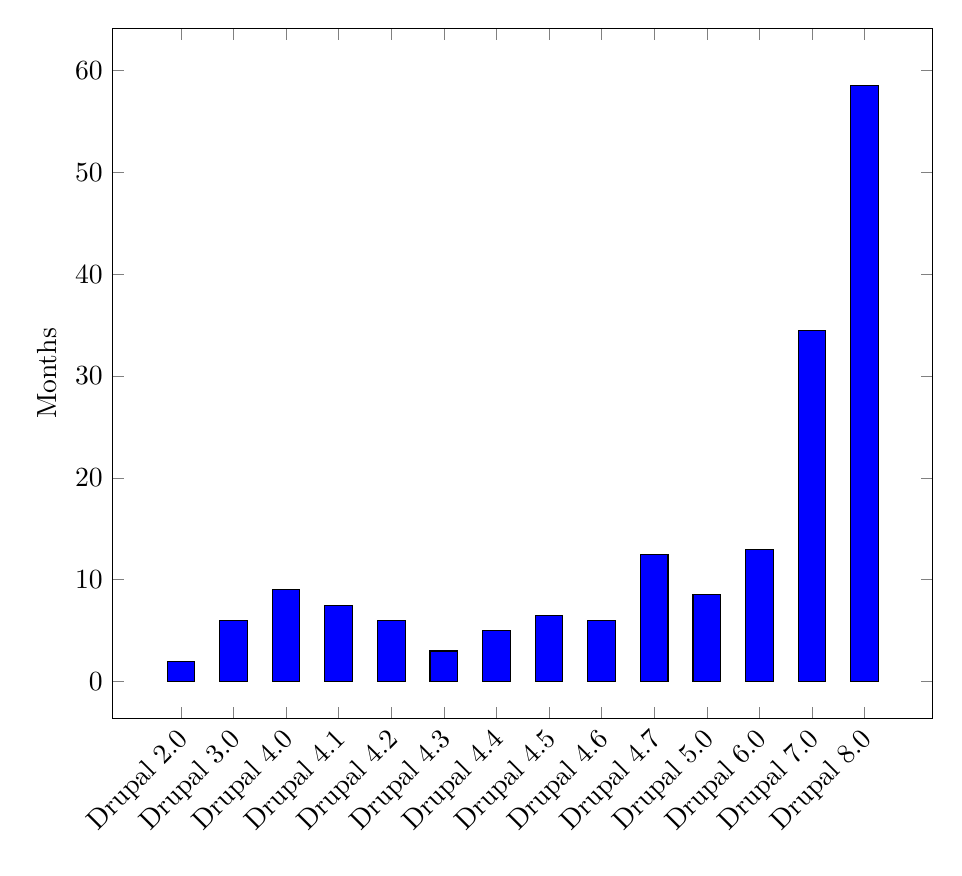
\begin{tikzpicture}
\begin{axis}[width=12cm,
    symbolic x coords={Drupal 2.0, Drupal 3.0, Drupal 4.0, Drupal 4.1, Drupal 4.2, Drupal 4.3, Drupal 4.4, Drupal 4.5, Drupal 4.6, Drupal 4.7, Drupal 5.0, Drupal 6.0, Drupal 7.0, Drupal 8.0},
    xtick=data,
    x tick label style={rotate=45, anchor=east, align=center, yshift=-5pt},
   % label style={font=\tiny},
    ylabel= Months]
    \addplot[ybar,fill=blue] coordinates {
(Drupal 2.0,2) (Drupal 3.0,6) (Drupal 4.0, 9)(Drupal 4.1,7.5) (Drupal 4.2,6) (Drupal 4.3,3) (Drupal 4.4,5) (Drupal 4.5,6.5) (Drupal 4.6,6) (Drupal 4.7,12.5) (Drupal 5.0,8.5) (Drupal 6.0,13) (Drupal 7.0,34.5) (Drupal 8.0,58.5)
    };
\end{axis}
\end{tikzpicture}
	\caption[Total amount of months between major releases]%
	{Number of months between major releases (see footnote \ref{numbering-conventions} to clarify the differences in the numbering conventions). Based on data collected by \textcite{zoubi-history:2016:Online}, under a CC BY-SA 2.0 license.}
	\label{stats-drupal-release}
\end{figure}

It is within this period that this study was carried out, hence, the main events and development that took place in this time will be extensively presented and analysed throughout this thesis. Nevertheless, some of the aspects that characterised this period should be introduced to provide a general overview of the key moments in the history of Drupal and its community. 

In addition to the continued growth in the adoption of Drupal and participation in the project, this period was characterised by a significant change in the organisational processes surrounding the development of version 8 of Drupal core. Figure \ref{drupal-8-core-release} provides an overview of the release cycle of Drupal applied for Drupal 8 \parencite{drupal-core-release-cycle:2014:Online} depicting, for example, clearer stages with regard to the scope of possible technical changes to be included. These stages were defined with the aim of improving coordination and synchronisation to solve dependencies during development. For instance, once the project entered a ``freezing" stage, new features could not be added. Another example of these changes towards a more structured set of processes was the introduction of the notion of ``Core Initiatives"\footnote{Core Initiatives, as well as other relevant organisational changes in the development of core, are extensively discussed and analysed in chapter \ref{chapter:core-system}.} \parencite{drupal-core-initiatives:Online}. The development was divided into several initiatives which were led either by a well-known developer in the community \parencite{drupal-core-initiatives:Online} appointed by Dries or by emergent groups whose proposals were required to fulfil a set of quality control criteria. These initiatives were considered high priority tasks by the community, and included for instance a new theme engine, the inclusion of multilingual capabilities that removed the need for \textit{contributed} modules, and the implementation of web services to allow Drupal to interoperate easily with other systems.

\begin{figure}[H]
	\centering
	\includegraphics[scale=0.8]{img/d8_release_cycle.png}
	\caption[Drupal 8 core release cycle]%
	{Drupal 8 core release cycle. Retrieved \nth{22} September 2014, from \url{https://drupal.org/files/d8_release_cycle.pdf}, under a CC BY-SA 2.0 license.}
	\label{drupal-8-core-release}
\end{figure}

Another key aspect to be highlighted during this period were the substantial technical changes carried out in the architecture, as well as the tensions created in the community as a consequence. The most prominent discussion was focussed on the inclusion of some components of the web application framework Symfony\footnote{Symfony is a FLOSS web application framework based on PHP \parencite{symfony:2017:Online}. It is characterised by a high degree of re-usability and modularity, drawing on other PHP FLOSS components. When compared with Drupal, Symfony's scope is of a lower level of abstraction. For example, it provides more control to the developer, but it requires more effort in writing customised code.} into Drupal's core, which originated in one of the Core Initiatives \parencite{drupal-8-symfony-webservices:2017:Online, drupal-8-symfony-webservices2:2017:Online}. This was also seen as an opportunity to change other major architectural aspects. For example, with regard to the way Drupalistas can interact with the core of the system, since it provided a way to deprecate\footnote{\label{deprecate}In software engineering, deprecated functions or features refers to those that are in the process of being replaced by newer ones \parencite{deprecate:2017:Online}.} the ``hooks system\footnote{As previously discussed in section \ref{sec:what-is-drupal}, hooks are the main means by which modules interact with Drupal core up to version 7 \parencite{drupal-hooks:2016:Online}.}".

Furthermore, these architectural changes did not only have technical consequences, but they could also have potential social ones, since they could affect the nature of the community and the participation in the project. On one hand, the benefits for the community of this new approach were argued for \parencite{drupal-symfony-announcement:Online} on the basis of what was known as the need to ``get off the island" \parencite{getting-off-island:2017:Online}: by following a paradigm similar to that of other PHP frameworks this could attract new PHP developers into Drupal, since it signified the end of a very specific Drupal paradigm which was in part causing the previously discussed ``hard learning curve". On the other hand, other Drupalistas argued that this could cause a ``loss of the hobbysts" in Drupal 8. From the point of view of these Drupalistas, this could produce a loss of the ``hacky" spirit which was the essence of Drupal's technical philosophy. They argued that this ``hacky" spirit embedded in the technology was one of the main reasons why amateurs had been able to experiment and customise Drupal's code easily, and it would especially affect them. In addition, they based their argument on the increment in the shaping of Drupal's architecture towards targeting larger projects, typically carried out by large corporations and the possible interest they may have in changing the project's technical direction \parencite{Rogers2014, kein-debate-1:2014:Online, kein-debate-2:2014:Online}. 

In the end Symfony was included and the ``hooks system" was deprecated\footnote{See previous foonote \ref{deprecate}.}, but the tension surrounding these important and significant technical changes would cause the creation of the first fork of Drupal by a group of Drupalistas: Backdrop\footnote{The main website of the project can be found at \url{https://backdropcms.org}.}. Their intention was announced on 21st August 2013 \parencite{drupal-backdrop:Online}, and they argued in favour of forking on the basis that Backdrop would help to maintain the amateur audience, since the new version of Drupal was oriented to the professional market. The relationships between the Drupal and Backdrop projects were and remain amicable. For example, it is common to find Backdrop developers at Drupal events to present and discuss the project. Nevertheless, the issue remains controversial at times, due to the fear of causing a division in the community. Despite the fork, Drupal 8 was finally released on \nth{19} November 2015 \parencite{d8-release:Online} after five years of development.

\section{The growth of the community}
\label{sec:growth-community}

As previously discussed, the significant growth experienced by the Drupal community is fundamental to contextualise this case study. Considering its size --- more than 1.3 million people registered on Drupal.org --- , the Drupal community cannot be understood as a representative example of either CBPP or FLOSS communities, since most of these communities are of a smaller scale in terms of participants, as it was discussed in chapter \ref{chapter:introduction}. For instance, drawing on the data of Ohloh.net\footnote{See section \ref{subsec:floss-tools}.}, \textcite{oss-size:2017:Online} estimated that 87\% of FLOSS projects have five or fewer committers per year, with only a 0.1\% of them having 200 or more. Thus, this case study should be understood as extreme: a case of a large and global Commons-Based Peer Production community, for which the study of how its self-organisational processes emerged, evolved and scaled up over time, will help to improve our understanding of the phenomenon of Commons-Based Peer Production. The focus in this study will be placed on the effects of this growth on the self-organisational processes of the community rather than on the reasons why this growth occurred, an aspect which would require an in-depth study in itself, and hence was concluded to be out of the scope of this thesis. To this end, this section is devoted to providing a more detailed discussion of the growth experienced by the Drupal community, by presenting and analysing some indicators of this growth in online and offline medium\footnote{Indeed, the online\slash offline distinction within this case study is blurred, and it should be understood as non-binary. These aspects are widely explored in chapter \ref{chapter:methods}, in which the sampling strategy is defined according to a spectrum comprised of ``mostly-online" and ``mostly-offline" contribution activities, on the basis of the medium in which the majority of actions and operations occurred. Nevertheless, in this chapter they are presented as online and offline for simplification purposes.}. The inclusion and comparison in this study of offline activities with equal relevance as online is another novel aspect of this research, since literature on FLOSS has tended to focus on online activities\footnote{These aspects will be explored more extensively in chapter \ref{identifyng-contribution:chapter}, where it is argued that this also relates to the need to broaden our understanding of contribution activities beyond those whose main focus of action is directed towards the digital commons themselves (e.g. writing code or documentation).}.

Regarding online activity, the Drupal community has been undergoing a process of significant growth throughout its existence. This is illustrated by various indicators, such as the increase in the number of users registered at Drupal.org and their increased participation in online activities.

With regard to the number of contributors, a simple indicator of this growth is the surpassing of the million mark of registered users in the main collaboration platform in October 2013 \parencite{drupalorg-1-million:2016:Online}. It is important to notice that this does not imply that all of these Drupalistas will become active contributors, or active in a similar way. As found in many other CBPP communities, an unequal distribution in the degree of participation is regularly found in CBPP. For instance, as found by \textcite{p2pvalue-del12:Online} in their quantitative study of more than 300 cases of CBPP, there is a tendency towards a 90-9-1 distribution power law with regard to participation: 90\% of the participants have a low level of engagement, around 9\% make minor contributions and around 1\% are very active contributors. Hence, as expected from a distribution with these characteristics, the total growth of the community\footnote{The methodological approach followed in this study, based on qualitative methods as will be discussed in chapter \ref{chapter:methods}, makes it difficult to offer a solid argument in terms of generalisation of whether Drupal does or does not follow a 90/9/1 distribution of participation. Nevertheless, the data reported by the community for online activities, as well as the observations carried out by the researcher or the qualitative interviews for offline activities --- whose indicators are less precise ---  were in line with this usual type of distribution with regard to the level of participation found in CBPP communities.} also encompasses a growth in the number of contributors which fall within these different levels of participation. For example, figure \ref{core-committers-release} depicts the number of Drupalistas who carried out at least one commit in Drupal core at the time of each major release, showing, for example, how the number of committers to core in Drupal 8 was more than three times the number of committers in Drupal 7 \parencite{drupal-cores:2016:Online, drupal7-core:2016:Online}.

% Plot for log10 core committers per release
\begin{figure}[H]
\centering
 \begin{tikzpicture}
  \begin{axis}[width=12cm, date coordinates in=x,date ZERO=2001-01-01,
               xticklabel=\year-\month-\day,ymin=0,ymax=4,
               x tick label style={rotate=45, anchor=east, align=center, yshift=-5pt},
               label style={font=\tiny},
       xmin=2001-01-01,
       xmax=2016-11-19]
   \addplot coordinates {
(2001-01-15,0)
(2001-03-15,0.7781512504)
(2005-04-15,1.698970004)
(2006-05-01,2.5289167)
(2007-01-15,2.673941999)
(2008-02-13,2.869818208)
(2011-01-05,2.979548375)
(2015-11-19,3.517195898)
   };

\addplot[mark=*] coordinates {(2001-01-15,0)} node[pin=45:{$(v1.0)$}]{} ;
\addplot[mark=*] coordinates {(2001-03-15,0.7781512504)} node[pin=0:{$(v2.0)$}]{} ;
\addplot[mark=*] coordinates {(2005-04-15,1.698970004)} node[pin=-75:{$(v4.6)$}]{} ;
\addplot[mark=*] coordinates {(2006-05-01,2.5289167)} node[pin=-30:{$(v4.7)$}]{} ;
\addplot[mark=*] coordinates {(2007-01-15,2.673941999)} node[pin=-170:{$(v5.0)$}]{} ;
\addplot[mark=*] coordinates {(2008-02-13,2.869818208)} node[pin=100:{$(v6.0)$}]{} ;
\addplot[mark=*] coordinates {(2011-01-05,2.979548375)} node[pin=-100:{$(v7.0)$}]{} ;
\addplot[mark=*] coordinates {(2015-11-19,3.517195898)} node[pin=-100:{$(v8.0)$}]{} ;
\legend{Core committers (log 10)}
\end{axis}
\end{tikzpicture}
	\caption[Number of core committers per release]%
    {Number of core committers (log 10) per release. Based on data collected by \textcite{zoubi-history:2016:Online}. The statistics from Drupal 3.0 to 4.5 could not be found, and they have been omitted. Retrieved \nth{10} March 2016, from \url{http://websolutions.hr/drupal-history}, under a CC BY-SA 2.0 license.}
	\label{core-committers-release}
\end{figure}

A similar sustained growth can be found with respect to the production of \textit{contributed} projects. Figure \ref{contrib-modules-release} depicts the emergence of this pool over several releases, illustrating this growth\footnote{This data might not be completely accurate. In this case, the source of the data is \textcite{zoubi-history:2016:Online}, who estimated it using the closest existing captures from web.archive.org for each release (e.g. \url{http://web.archive.org/web/20041205054156/http://cvs.drupal.org/viewcvs/drupal/contributions/modules/}). In addition, it is also important to remark that unfortunately the number of Drupalistas with permissions to commit over time could not be recovered. Nevertheless, as in the previous cases, the use of figures is intended to illustrate the clear growth of the community, rather than to carry out a detailed analysis which a more quantitative approach would require.}.

% Plot for log10 contributed modules per release
\begin{figure}[H]
\centering
 \begin{tikzpicture}
  \begin{axis}[width=12cm, date coordinates in=x,date ZERO=2001-01-01,
               xticklabel=\year-\month-\day,ymin=0,ymax=5,
               x tick label style={rotate=45, anchor=east, align=center, yshift=-5pt},
               label style={font=\tiny},
       xmin=2001-01-01,
       xmax=2016-03-10]
   \addplot coordinates {
(2001-01-15,0)
(2002-06-15,0.6020599913)
(2003-02-01,0.6989700043)
(2003-08-01,0.84509804)
(2003-11-01,0.6020599913)
(2004-04-01,0.903089987)
(2004-10-18,2.471291711)
(2005-04-15,2.525044807)
(2006-05-01,2.88592634)
(2007-01-15,3.419294722)
(2008-02-13,3.864629725)
(2011-01-05,4.066586796)
(2015-11-19,3.430236353)
   };
   
\addplot[mark=*] coordinates {(2001-01-15,0)} node[pin=25:{$(v1.0)$}]{} ;
\addplot[mark=*] coordinates {(2002-06-15,0.6020599913)} node[pin=-270:{$(v4.0)$}]{} ;
\addplot[mark=*] coordinates {(2003-02-01,0.6989700043)} node[pin=0:{$(v4.1)$}]{} ;
\addplot[mark=*] coordinates {(2003-08-01,0.84509804)} node[pin=-270:{$(v4.2)$}]{} ;
\addplot[mark=*] coordinates {(2003-11-01,0.6020599913)} node[pin=-20:{$(v4.3)$}]{} ;
\addplot[mark=*] coordinates {(2004-04-01,0.903089987)} node[pin=45:{$(v4.4)$}]{} ;
\addplot[mark=*] coordinates {(2004-10-18,2.471291711)} node[pin=-150:{$(v4.5)$}]{} ;
\addplot[mark=*] coordinates {(2005-04-15,2.525044807)} node[pin=-75:{$(v4.6)$}]{} ;
\addplot[mark=*] coordinates {(2006-05-01,2.88592634)} node[pin=-30:{$(v4.7)$}]{} ;
\addplot[mark=*] coordinates {(2007-01-15,3.419294722)} node[pin=-170:{$(v5.0)$}]{} ;
\addplot[mark=*] coordinates {(2008-02-13,3.864629725)} node[pin=145:{$(v6.0)$}]{} ;
\addplot[mark=*] coordinates {(2011-01-05,4.066586796)} node[pin=-100:{$(v7.0)$}]{} ;
\addplot[mark=*] coordinates {(2015-11-19,3.430236353)} node[pin=-100:{$(v8.0)$}]{} ;   
   
\legend{\textit{Contributed} projects (log 10)}
\end{axis}
\end{tikzpicture}
	\caption[Number of \textit{contributed} projects per release]%
    {Number of \textit{contributed} projects (log 10) per release. Based on data collected by \textcite{zoubi-history:2016:Online}, drawing on captures from web.archive.org. The statistics from Drupal 2.0 and 3.0 could not be found, and they have been omitted. Retrieved \nth{10} March 2016, from \url{http://websolutions.hr/drupal-history}, under a CC BY-SA 2.0 license.}
	\label{contrib-modules-release}
\end{figure}

The figure depicts constant growth, with the exception of the difference between Drupal 8 with respect to Drupal 7. This difference can be explained, however, by the time at which the data for Drupal 8 was collected, and the large difference in the period to develop modules between major releases. Contributed projects typically start to be developed and ported once the final release has been made, or some months before. Hence, the numbers refer to a period of approximately thirteen months since the release. A similar reason can explain the lower amount of contributed modules for Drupal 4.3 with respect to 4.2, since the difference between releases was three months (see figure \ref{stats-drupal-release}).

In a similar way as in the case of online activities, the Drupal community has experienced a significant growth in the organisation of offline activities and participation in them. The first international F2F meeting in Belgium in 2005\footnote{See section \ref{subsec:offline-side}.} would be a source of inspiration for the emergence and spread of a wide range of different types of F2F events, ranging from local events focussed on presentations, sprints to contribute back to the community or simply informal meetings for drinks with other Drupalistas, to events whose organisational dynamics more closely resemble those of conferences. For example, \textit{DrupalCons} (see figure \ref{drupalcon-amsterdam-2014}): major international Drupal events which take place over the course of a week. They include peer-reviewed presentations, more informal presentations or ``BoFs" (Birds of a Feather), community summits, code sprints, social events and public Drupal Association meetings, to name but a few activities. They are organised by the Drupal Association\footnote{The organisational changes experienced over time will be extensively discussed in chapter \ref{mostly-offline-cons:chapter}.}, with the support of the local community of the city in which it is held. They are commonly organised on a yearly basis at a continental level: originally in North America and Europe, although more recently there were first editions in Australia (2013) \parencite{drupalcon-aus:2016:Online}, South America (2015) \parencite{drupalcon-sa:2016:Online}, and Asia (2015) \parencite{drupalcon-asia:2016:Online}. Attendance fees are significantly costly, around the hundreds of euros\slash dollars. For instance, the price of a regular ticket for the whole event at \textit{DrupalCon} Amsterdam 2014 was 500\euro{}.


\begin{figure}[H]
	\centering
	\includegraphics[scale=0.32]{img/events/drupalcon_human_drop.jpg}
	\caption[\textit{DrupalCon} Amsterdam 2014]%
    {Group picture at \textit{DrupalCon} Amsterdam 2014, which attracted more than 2,000 participants. The group is forming a ``human drop" resembling Druplicon, the logo of Drupal (see figure \ref{druplicon}). Retrieved \nth{13} November 2014, from \url{http://chapterthree.com/blog/chapter-three-drupalcon-amsterdam}.}
	\label{drupalcon-amsterdam-2014}
\end{figure}

The growth of offline participation can be observed using indicators such as attendance to these \textit{DrupalCons}. For example, figure \ref{dcons-eu-na} depicts the overall growth in the number of attendees in Drupalcons held in Europe\footnote{The data from the two events in 2005 might not be as accurate as the rest. It is indicated as \textless 50 and approximately 100. Hence, those estimated figures (50 and 100) have been employed for the coordinates chart, and combined within the same year in the graph but depicted by a line. It is also important to notice that the first \textit{DrupalCon} event in Europe was organised in 2007. The previous events were part of major FLOSS conferences, such as FOSDEM. In any case, the figures are useful to provide an overview of the growth, since they refer specifically to attendance of Drupalistas.} and North America\footnote{The data from 2005, 2006 and 2007 may not be as accurate as the rest. It is indicated as \textgreater 100, approximately 150 and \textgreater 300 respectively. Hence, those estimated figures (100, 150 and 300) have been employed for the chart.  It is also important to notice that, according to the documentary analysis  \parencite{drupalcon-vancouver:2016:Online}, the first specific \textit{DrupalCon} event in North America was organised in 2006 in Vancouver.  Nevertheless, experienced Drupalistas who were interviewed explained that the \textit{DrupalCon} in Boston (2008) should be considered the closest to what is now considered a \textit{DrupalCon}. Previous events (including 2007) were part of major FLOSS conferences, such as OSCOM (Open Source Convention). In any case, the figures are useful to provide an overview of the growth, since they refer specifically to attendance of Drupalistas.}.



%Plot combining attendance to DrupalCon Europe and DrupalCon America
\begin{figure}[H]
\centering
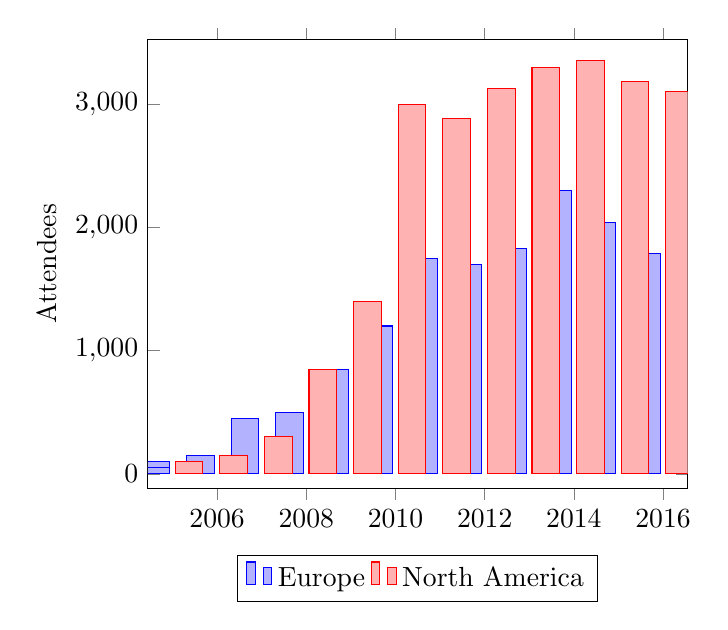
\begin{tikzpicture}
\begin{axis}[
	x tick label style={
		/pgf/number format/1000 sep=},
	ylabel=Attendees,
	enlargelimits=0.05,
	legend style={at={(0.5,-0.15)},
	anchor=north,legend columns=-1},
	ybar,
]
\addplot 
	coordinates {(2005,50)(2005,100) (2006,150) (2007,450) (2008,500) (2009,850) (2010,1200) (2011,1751) (2012,1700) (2013,1830) (2014,2300) (2015,2039) (2016,1787)};
\addplot 
	coordinates {(2005,100) (2006,150) (2007,300) (2008,850) (2009,1400) (2010,3000) (2011,2881) (2012,3127) (2013,3300) (2014,3357) (2015,3186) (2016,3102)};
\legend{Europe,North America}
\end{axis}
\end{tikzpicture}
\caption[Number of attendees to \textit{DrupalCon} events in Europe and North America]%
    {Number of attendees to \textit{DrupalCon} events in Europe and North America. Based on data reported by the \textcite{drupal-association-dcons-attendance:2016:Online}.}
	\label{dcons-eu-na}
\end{figure}

The growth in the participation of Drupalistas in \textit{DrupalCons} was particularly significant in the periods 2008-2011 for the case of Europe and 2008-2010 for the case of North America. As it will be discussed in section \ref{subsec:dcons-growth}, this was a clear point of change with regard to the organisational processes of \textit{DrupalCons}. There were slight decreases with respect to the previous edition in 2011 for the case of North America, and in 2012 for the case of Europe. However, after those editions growth continued. Nevertheless, the most recent editions (2015 and 2016) depict a more prominent decline in attendance. This has awoken concern in the community, and it is commonly explained by Drupalistas as a loss of momentum in adopting Drupal due to the long time (five years) which it had taken to develop Drupal 8 \parencite{drupal-momentum:2016:Online}, in a similar way as the previous decline after Drupal 7\footnote{An in-depth analysis of this aspect was beyond the scope of this study. Other hypothesis could be based on a reduction in the rate of growth, as in the case of Wikipedia \parencite{suh2009singularity}, or the impact of the fork described in section \ref{subsec:d7-d8}.}.

Other indicators of this growth can be found in the growing numbers of \textit{DrupalCamps}\footnote{\label{fn-dev-days}In addition to \textit{DrupalCamps}, events specialised in specific roles, a topic that will be more extensively discussed in section \ref{par:roles},  such as Drupal Dev Days --- aimed at backend developers --- or Frontend United --- aimed at themers --- are also held by the community. While they were distinctively considered during certain stages of this study --- for example while studying the notion of contribution in chapter \ref{identifyng-contribution:chapter} --- they are included as part of this category in this classification for simplification purposes because of their similarities in organisational dynamics.} (see figure \ref{drupalcamp-spain-2014}): for example, while in 2007 six \textit{DrupalCamps} were organised, the number ascended to 67 in 2013 \parencite{ostraining-list-drupalcamps:2016:Online}. These are two or three day events focussing on sharing knowledge within the community. They include peer-reviewed  presentations, Drupal sprints and social events. They are frequently organised once a year, typically at a national level. However, in large countries or those countries with the largest Drupal communities they are organised regionally. For example, in the case of the UK there are events such as \textit{DrupalCamp} London, \textit{DrupalCamp} North West, \textit{DrupalCamp} North East, \textit{DrupalCamp} Brighton and \textit{DrupalCamp} Bristol. They are organised by local communities, and their attendance requires a relatively low fee which depends on the country (e.g. for the UK around 30-40\pounds). Their levels of attendance vary, but it is commonly around the hundreds. For example, events which have been held for consecutive years tend to attract around 200-300 people.

\begin{figure}[H]
	\centering
	\includegraphics[scale=0.37]{img/events/drupalcamp_spain.jpg}
	\caption[\textit{DrupalCamp} Spain 2014]%
    {Group picture at \textit{DrupalCamp} Spain 2014 (May). Retrieved \nth{9} July 2014, from \url{http://2014.drupalcamp.es}.}
	\label{drupalcamp-spain-2014}
\end{figure}

Similar indicators of this growth can be found in the case of local events\footnote{An exhaustive list of all these events over time does not exist, to the best of my knowledge. The most precise source found is \url{https://groups.drupal.org/events}. It operates as a wiki in which Drupalistas add some of the events. The collected data is employed by other sites, as in the case of the presented World map visualisation by \textcite{drupical:2016:Online}. However, it is important to notice that this list may not be completely accurate. For example, one of the smaller local events which I attended, organised via Meetup.com, was not included within this data. In addition, external sources such as \textcite{ostraining-list-drupalcamps:2016:Online} were employed, since they provide a historical archive. However, they are also limited. For example, in the event referred to the collection of data stopped in 2013.}, or the nearly 600 regional groups listed at Drupal.org \parencite{drupalorg-groups:2016:Online}. For instance, tens of local Drupal meetups are held every month worldwide: a filtered list of local events in Drupical \parencite{drupical:2016:Online} displays 38 events (see figure \ref{drupical-local-events}) being organised in a month's time. 

\begin{figure}[H]
	\centering
	\includegraphics[scale=0.25]{img/offline/drupical_march_2017}
	\caption[World map of Drupal local events]%
    {Forthcoming Drupal local events in a month's time at the time of writing (01/03/2017). Screenshot from Drupical.com. Retrieved \nth{01} March 2017, from \url{http://www.drupical.com}.}
	\label{drupical-local-events}
\end{figure}

The characteristics and functions of these local events differ significantly in their purpose and level of formality: from the most informal and social events (Drupal Beer and Chat), to those focussed on presentations on case studies or the technical advances of the platform for learning purposes (Drupal Show and Tell). For example, the following local events were studied as part of this research:

\textbf{Drupal Beer and Chat\footnote{The names given by Drupalistas to all these events differ in different local communities. For example, in Spanish local communities similar events are commonly known as ``Drupaladas".}}

These are considerably informal events in which people with an interest in Drupal meet in a pub to discuss Drupal, without an agenda. In the case of the observation in London, they commonly started around 7pm, and finished once the pub was closed, typically 11pm to 12am. They attracted tens of people --- an average of 15 to 20 during observations --- and were mainly organised via Meetup.com\footnote{\url{http://www.meetup.com/London-Drupal-Pub-Meet/}, accessed on \nth{14} November 2014.}. They were organised approximately once a month.

\textbf{Drupal Show and Tell}

These are informal presentations about diverse topics in Drupal, such as case studies, presenting new technologies and modules, and sessions to advise on the implementation of certain functionalities (see figure \ref{drupal-show-tell}). In the case of the observations carried out in London, they typically started at 6pm, and concluded within 1.5 or 2 hours. They were held in rooms which enabled the use of slides (e.g. universities and company meeting rooms). After the event, there was commonly a more informal meeting, whose dynamics were similar to those of a Drupal Beer and Chat. They also attracted tens of people --- typically between 25 to 35 --- and were similarly organised via Meetup.com\footnote{\url{http://www.meetup.com/drupal-show-and-tell/}, accessed on \nth{14} November 2014.}  and mailing lists. They were organised approximately once a month.

\begin{figure}[H]
	\centering
	\includegraphics[scale=0.09]{img/offline/drupal_show_tell_london.jpg}
	\caption[London Drupal Show and Tell]%
    {Picture from a London Drupal Show and Tell in January 2016. Retrieved \nth{17} January 2016, from \url{https://www.meetup.com/drupal-show-and-tell/photos/26670134/445910901/}. Chandeep Khosa.}
	\label{drupal-show-tell}
\end{figure}

\textbf{Drupal Sprint}

These are events focussed on contributing back to the Drupal community, with organisational dynamics similar to those of ``hackathons" \parencite{lapp20072006}. Their participants collaborate to write software, documentation or carry out testing, among other activities (see figure \ref{drupal-sprint-weekend}). Additionally, there are sometimes Drupal training sessions to help newcomers to start contributing (Drupal Ladders\footnote{\url{http://drupalladder.org/}, accessed on \nth{14} November 2014.}). In the case of London, these events typically took place throughout whole weekends, starting at around 10am and finishing around 6pm. They were held in ``open spaces" rooms, where participants could bring their laptops and sit next to each other to collaborate. During observation, they attracted around 10-20 people. They were mainly organised via EventBrite\footnote{\url{http://www.eventbrite.co.uk/o/drupal-london-community-61878136}, accessed on \nth{14} November 2014.}, but also promoted via Drupal.org. They were organised once a month approximately.

\begin{figure}[H]
	\centering
	\includegraphics[scale=0.55]{img/events/drupal_coding_sprint.jpg}
	\caption[Drupal Sprint Weekend]%
    {Picture from a Drupal Sprint Weekend, to promote a new event in April 2014. Retrieved \nth{27} August 2014, from \url{https://groups.drupal.org/node/416908}, under a CC BY-SA 2.0 license.}
	\label{drupal-sprint-weekend}
\end{figure}

\textbf{Drupal Coworking Day}

These are informal events where Drupal professionals, typically freelancers, but also people working for companies, meet to work together or ``coworking" \parencite{spinuzzi2012working} and help each other with their personal or professional Drupal projects. For instance, in observations in London these events took place during workdays, starting at around 10am and finishing at around 5pm. Although, as with the events previously described, there was no cost for attendance, in this case they required a RSVP due to limits in the number of places --- ten for this specific case. They were mainly organised via Meetup.com\footnote{\url{http://www.meetup.com/London-Drupal-Coworking-Meetup}, accessed on \nth{14} November 2014.}, and held approximately twice a month.

Overall, the previous indicators illustrate the significant growth experienced by the community over time, while the concrete examples illustrate its diversity. In the next section another relevant aspect is discussed, that of ``do-ocracy" in relation to the culture of the community.

\section{Life in a ``do-ocracy": a model of governance?}
\label{sec:do-ocracy}

When asked about the model of governance of the Drupal project, Drupalistas commonly defined it as a ``do-ocracy". ``Do-ocracy" is a notion that encourages open participation. It is based on the self-allocation of tasks, and it allows those who carry out these tasks to be recognised and become more influential in order to make decisions when ``rough consensus" \parencite{russell2006rough} is necessary to be reached. The following excerpt from Dries \parencite[514]{bacon2012art}, the original creator of Drupal, illustrates how these main characteristics of ``do-ocracy" shape the day-to-day life of the Drupal community:

\begin{quotation}
``[...] The Drupal community uses a ``do-ocracy" model, meaning people work on what they want to work on, instead of being told what to work on. Decisions are usually made through consensus building and based on technical merit, trust and respect."
\end{quotation}

Not surprisingly, the notion of ``do-ocracy" presents characteristics that resemble those of the hacker culture discussed in section \ref{subsec:hacker}. For example, in relying on meritocratic values --- such as the ``technical merit" mentioned in the quote above --- and encouraging the focus to be placed on contribution activities and quality, rather than on the personal characteristics of those who carry them out --- ``Hackers should be judged by their hacking, not criteria such as degrees, age, race, sex, or position" \parencite[35]{levy1984hackers}. Another example is the mistrust of formal authority, as part of a more general anti-bureaucratic attitude of hackers. A ``do-ocracy" operates on the idea that those who mobilise more resources towards a certain task and demonstrate their merit to the community have the legitimacy to make decisions that relate to that task, rather than legitimacy being based on arbitrary rules that consolidate power representing a threat for their creative impulses \parencite[25]{levy1984hackers}.

The notion of ``do-ocracy" is commonly found to describe the governance of organisational processes of CBPP communities \parencite[e.g.][]{mateos2008institutions, fuster2010governance, zacchiroli2011debian, kostakis2014production}. For example, \textcite[282]{fuster2010governance} incorporated this notion in the context of the study of the governance of online creation communities and defined it as follows:

\begin{quotation}
``[...] Doocracy refers to the idea that there is no external body or hierarchy that decides how actions should be carried out. In other words, in a doocracy authority over an action is held directly by those developing it. Furthermore, participants gain influence and authority in the process according to their merits and the resources for `doing' that they mobilize (such as time or attention)."
\end{quotation}

In addition, these ``do-ocratic" characteristics incorporate numerous similarities with those presented in the literature review of governance of CBPP communities in section \ref{subsec:governance-cbpp}, such as the attributes defined by \textcite{benkler2006commons}. The previous quote by Dries depicts, for example, the self-assignation of tasks, whose outcomes' quality is scrutinised through peer-reviewing processes carried out by the community.

Nevertheless, these ``do-ocratic" characteristics also imply an inherently blurred and informal nature, which can become a source of inner contradictions and tensions as communities adapt their self-organisational processes over time. For instance, the willingness to decentralise the governance of the community may produce tensions with respect to the rejection of bureaucratisation, since formal rules may be interpreted as arbitrary with the aim of consolidating power in the hackers' eyes.

In the case of the Drupal community similar tensions and inner contradictions emerged, for example, when the community grew and discussed the necessity to formalise the self-organisational processes to scale up. For instance, the following excerpt, from a post by Dries \parencite{do-ocracy01:2016:Online} in the context of a discussion about Drupal governance in March 2013, depicts some of these tensions and frustrations generated by a lack of clarity in certain processes, in this case those related to the governance of the main collaboration platform and the Drupal Association:

\begin{figure}[H]
  \centering
\includegraphics[scale=0.5]{img/quotes_replacement/do-ocracy-dries.png}
\caption[Excerpt from the article ``Creating a structure for Drupal governance"]{Excerpt from the article ``Creating a structure for Drupal governance". Retrieved \nth{27} July 2017, from \url{http://buytaert.net/creating-a-structure-for-drupal-governance}.}
\label{do-ocracy-dries}
\end{figure}

Hence, when applied to the model of governance of large and global CBPP communities, the notion of ``do-ocracy" lacks relevant aspects, such as the emergence of more formal organisational forms depicted, for example, by the numerous institutions created over time by the Drupal community. For this reason, this study incorporates the notion of ``do-ocracy" not as a model of governance, but as part of a strong culture within the Drupal community \parencite{melanccon2011contributing}, whose values are interrelated and influenced by the values of the hacker culture discussed in section \ref{subsec:hacker}. To this end, the model of governance is a subject matter of this study in itself, in which the influence of the ``do-ocratic" culture is considered as relevant in the shaping of the organisational processes of peer production over time, but assuming that, as shown in the literature review in chapter \ref{chapter:introduction}, there remains a necessity to improve our understanding of how large and global CBPP communities, such as Drupal, organise themselves and scale up while remaining viable over time.

Furthermore, this research conceptualised tensions\footnote{Further details about how the notion of tension is incorporated through the main theoretical framework employed in this study will be presented in chapter \ref{sec:theoretical-frameworks}.}, as those discussed between the anti-bureaucratic attitude and the formalisation of processes to decentralise the governance, as ``windows of opportunity" to follow and collect data during the study. Hence, these tensions will help to 
improve our understanding of the emergence of the processes and structures which the Drupal community has created over time. For example, to improve our understanding of how decentralisation, a key notion to be explored in CBPP as argued in chapter \ref{chapter:introduction}, occurred or whether it did. This study develops from the notion of decentralisation in the context of CBPP of \textcite[62]{benkler2006wealth} as the ``conditions under which the actions of many agents cohere and are effective despite the fact that they do not rely on reducing the number of people whose will counts to direct effective action", applying it to question whether decentralisation occurred in the peer production activities of the community and how it did. This was materialised, for example, by exploring how legitimacy emerged and changed over time in the community in order to decentralise decision-making to perform changes in the digital commons, or to organise events; or to analyse whether practices regarding decision-making related to quality assurance were decentralised and how this occurred.

Another example of opportunity for further study, which arose from the aforementioned tension, is to be found in the need to explore the changes experienced in the organisational processes over time and the organisational dynamics. As stated by \textcite[61]{benkler2006wealth}: ``the salient characteristic of commons, as opposed to property, is that no single person has exclusive control over the use and disposition of any particular resource in the commons. Instead, resources governed by commons may be used or disposed of by anyone among some (more ore less well-defined) number of persons, under rules that may range from `anything goes' to quite crisply articulated formal rules that are effectively enforced". As discussed in chapter \ref{chapter:introduction}, there is a lack, however, of an in-depth understanding of how these ``doocraticly-shaped" rules emerge, operate, are enforced and change over time in large communities, with the few exceptions of largely studied communities such as Wikipedia \parencite{viegas2007hidden, forte2009decentralization}.

This discussion of the notion of ``do-ocracy" concludes the introduction to the case study and the fundamental concepts that surround it in order to frame this research. With the aim of framing the previously discussed gaps in the literature into research questions, the next section presents the main research question and the research sub-questions tackled in this study.

\section{Research questions}
\label{subsubsec:state-art:drupal:case-study}

The main research question tackled in this study is as follows:

\emph{``How does a large and global Commons-Based Peer Production community self-organise?"}

The concepts of ``Commons-Based Peer production community", ``large" and ``global" have been discussed and framed within the context of this case study in chapters \ref{chapter:introduction} and \ref{chapter:case-study}, however, it is important to note that by ``self-organisation" the main research question draws on the efforts to explore the use of this concept within social science. Instead of relying on an undesirable monolithic definition of the concept  \parencite{gilbert2015self, anzola2016self}, this study develops from the notion of self-organisation characterised by four shared features within the literature suggested by \textcite{gilbert2015self}. Firstly, the formation of patterns, which are commonly ``designated by nominalised verbs" \parencite[4]{anzola2016self}. For example, in the case of Commons-Based Peer Production, ``cooperation\footnote{See section \ref{subsec:state-art:cbpp}.}". Secondly, the concept of autonomy, referring to the changes in the self-organisational system originating from the entities of the system or the interactions between them, rather than from a central source of control. For instance, this is depicted in the case of CBPP in the planification and execution of peer-production tasks in a decentralised manner\footnote{See section \ref{subsec:governance-cbpp}.}. Thirdly, referring to the robustness and resilience of self-organised systems, with respect to the ability of these systems to resist and to adapt to change respectively. This case study draws on this feature, for example, by incorporating tensions, as those originated by ``do-ocratic" and hacker culture\footnote{See section \ref{sec:do-ocracy}.}, as ``windows of opportunity" to follow and collect data during the study. Fourthly, dynamics, referring to the variation of the characteristics of self-organisational systems over time. For example, in this case study, carrying out the analysis of the self-organisational processes considering these variations, such as decentralisation of decision-making and formalisation. 

In addition, it is also important to remark that in order to tackle the main research question, a set of research sub-questions are also formulated and addressed in subsequent chapters.

Firstly, an essential element in order to frame the main research question through the study of the self-organisational processes themselves is related to the notion of contribution within FLOSS and CBPP communities. As it was presented in section \ref{subsubsec:state-art:floss:academic-research}, the studies which analyse the relationship between contribution and organisational aspects have typically focussed their attention on the most visible outcome of contribution: the collaboratively built shared objects. For instance, the most well-known type of contribution activity in FLOSS communities is the development of source code and, consequently, this has been typically the most studied. To this end, chapter \ref{identifyng-contribution:chapter} will present the findings regarding the exploration of this notion, helping to shed light on other activities that have not been widely studied due to their lack of visibility. This aspect is especially critical in a community that, as previously discussed, has been characterised as ``code-centric" \parencite{Zilouchian2011, Sims2013, nordinmotivation2014}.  Hence, this enables the identification and consideration throughout the study not only of the activities which are ``officially" understood as contributions, such as those listed in the main collaboration platform, but also of those which have remained less visible. The research sub-question that will be tackled during this chapter is as follows:

\emph{``What types of activities are understood as contributions in the Drupal community and in what ways are these recognised?"}

Secondly, once these contribution activities are identified, the focus of this thesis will shift towards improving our understanding of the main organisational aspects and dynamics that surround the development of these contribution activities. To this end, chapters \ref{sec:custom-to-contrib} to \ref{mostly-offline-cons:chapter} will address the study of the emergence of and changes in these self-organisational processes. The way in which the evolution of these processes responded to general organisational dynamics of formalisation and decentralisation in order to scale them up will then be discussed, as well as how these dynamics affected these processes to different degrees. To this end, the following research sub-questions will be tackled during these chapters:

\begin{itemize}
	 \item \emph{``What are the main organisational aspects and dynamics that have characterised the growth of a global CBPP community of such a scale?"}
	 \item \emph{``What type of governance emerged in the Drupal community?"}
\end{itemize}

Finally, once all these organisational aspects and dynamics have been extensively explored and analysed, the underpinnings to tackle the main research question are laid out. Thus, chapter \ref{multilevel:chapter} will address the main research question, providing a discussion of the central argument around the emergence of \textit{polycentric} governance as the main explanation in order to understand the manner in which the Drupal community has managed to self-organise while remaining viable, while contextualising the argument with respect to previous literature on Commons-Based Peer Production. The fundamental aim will be to offer an explanation of how Drupalistas have been able to organise themselves not just by one, but by multiple governing authorities at different levels varying in the degree of \textit{organicity}.

\section{Conclusion}

Throughout this chapter the fundamental aspects to contextualise the case study for this research were introduced. A brief historical overview of Drupal and its community was provided, illustrating the emergence and growth of a well-known case of Commons-Based Peer Production. This historical account should not be understood as exhaustive, but rather as an overview of the principal aspects necessary to frame this research, such as the increase in users, the emergence of more formal institutions and the tensions experienced as part of the growth of the community.

Among these aspects, two were more extensively discussed on the basis of their relevance for this research. Firstly, the growth experienced in participation in the community through both online and offline media. This aspect is key, since it provides an opportunity to explore organisational dynamics within the context of an extreme case study of Commons-Based Peer Production, hence enabling an improvement in our understanding of how these self-organisational processes emerge, evolve and scale up over time while remaining viable in these conditions. Secondly, the notion of ``do-ocracy" was explored and discussed. It was argued that, despite community accounts, this notion should not be understood as a model of governance since, although it is useful to understand certain characteristics of smaller CBPP communities, the use of the term ``do-ocracy" oversimplifies the complexity hidden behind the governance of the self-organisational processes within the case study. Instead, this study incorporates this notion --- the values  of which were argued to have been inspired by and subsumed within those of hacker culture --- as a relevant force in shaping the self-organisational processes of the Drupal community as well as its governance, but developing from the assumption that these issues require further exploration from a sociological perspective. In addition, the contradictions presented by some of the principles of these cultural forces, such as the tension between calls to formalise certain processes related to decision-making in order to decentralise them, and the common anti-bureaucratic attitude of hackers, were argued to be points of tension, the study of which will help the understanding of the emergence of organisational structures and processes in the community over time. To conclude, the research questions tackled in this study were presented.

With the aim of starting to address these questions, the next chapter will introduce the main theoretical framework employed in order to conceptualise this case study for its exploration: Activity Theory.